
%\textbf{Anschluss:} 

\begin{figure}[ht]
  \centering
  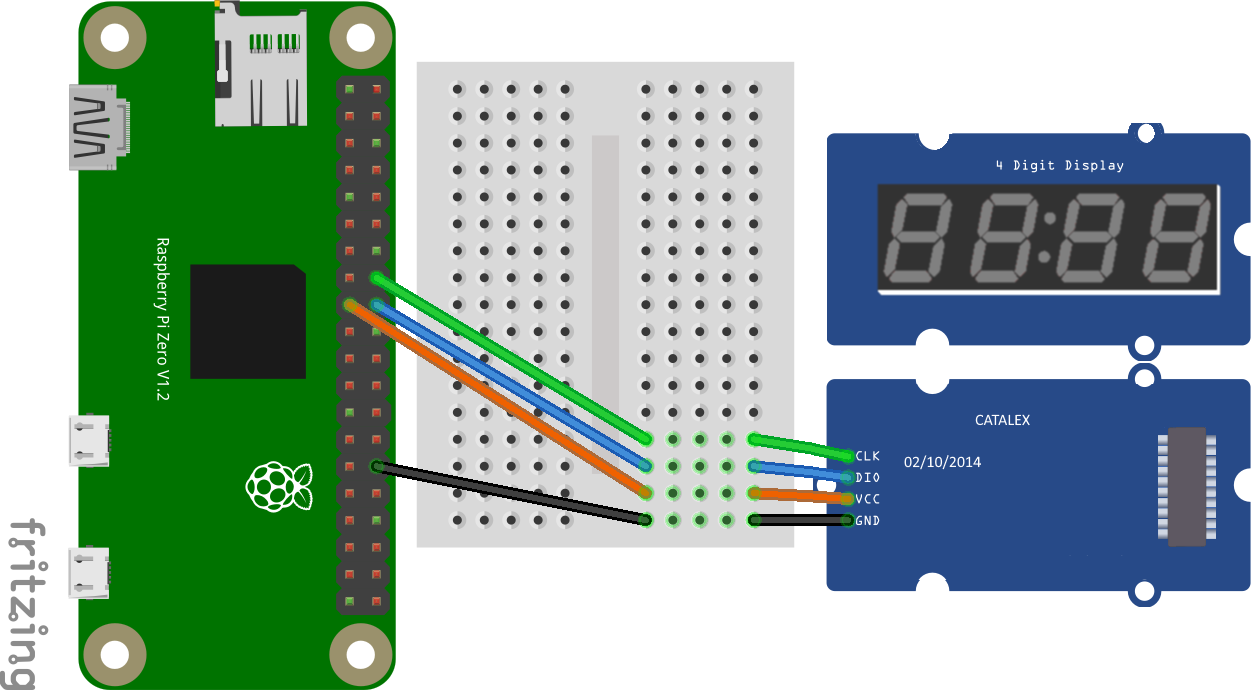
\includegraphics[scale=0.25]{images/TM1637_Steckplatine.png}	
  %	\caption{}
  \label{TM1637}
\end{figure}

\begin{figure}[ht]
	\centering
	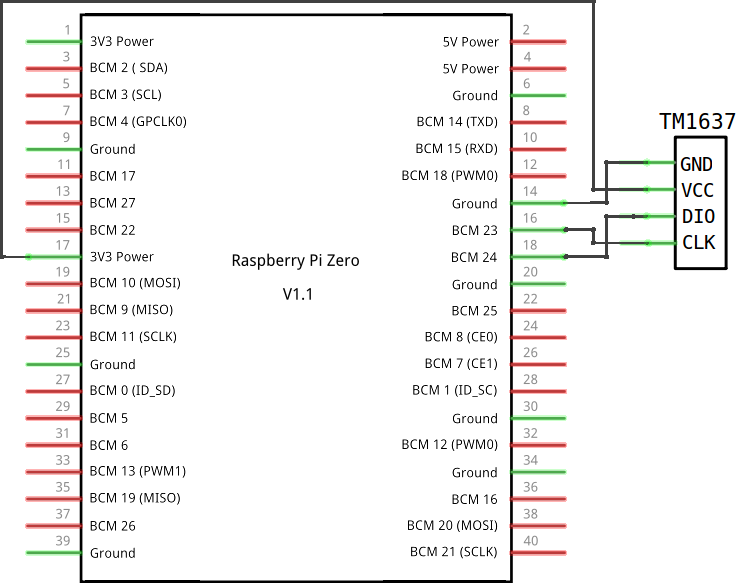
\includegraphics[scale=0.25]{images/TM1637_Schaltplan.png}	
	%	\caption{}
	\label{TM1637}
\end{figure}

\ExerciseBox{
Gib Zahlen und Texte aus [Beispiele]\\
Gib die aktuelle CPU Temperatur aus [Beispiel Python]\\
Gib die gemittelte aktuelle CPU Last in Prozent aus\\
Realisiere eine Laufschrift}

%https://www.mpja.com/download/31227sc.pdf

\textbf{C:} 

\begin{console}
	git clone https://github.com/mstroh76/TM1637Display
	cd TM1637Display
	g++ -o TM1637Display *.cpp -lwiringPi
	./TM1637Display
	geany project.geany & 
\end{console}

\textbf{C\#:}

\begin{console}
	git clone https://github.com/chirndler/wiringpi.net.sensors.git
	cd wiringpi.net.sensors
	xbuild /p:Configuration=Release wiringpi.net.sensors.sln
	cd bin/Release/
	sudo mono wiringpi.net.sensors.sample.exe 3
\end{console}

\clearpage
\textbf{Python:}
\begin{console}
	sudo pip3 install wiringpi
	git clone https://github.com/depklyon/raspberrypi-python-tm1637.git
	cd raspberrypi-python-tm1637
	sudo python3 setup.py install
\end{console}

\lstset{language=Python, caption=, 
        label=TM1637Program, frame=single, basicstyle=\ttfamily
	      \footnotesize, breakatwhitespace=false, showstringspaces=false, 
        showtabs=false, tabsize=2 }
\lstinputlisting{source/TM1637_Temp.py}

\begin{console}
	python3 TM1637_Temp.py
\end{console}